\subsection{Technology}
To implement all this algorithm I chosed to use Dart, which is a language developed and released recently by Google. Dart has the advantages to be used inside a command line interface (as a shell as we can use python script) or to be compiled to JavaScript for being used inside a website or a browser.\\
One of my idea was to develop the solution and then offer a website where it could have been possible to test the implementation directly.

\subsection{Lexer}
The lexer is the part, inside a parser, that will handle the first action of a parser : transform input characters into tokens. A simple definition of a token, in a parser, is a set of characters or tokens identified by a specific key, by example the token 'digit' will identify all the characters considered as digit as 0, 1, 2, ...\\
This task is done by Scanner. Scanner is a class that will handle the process of taking a parsing unit (here a character) inside a input (a string or a file) and return a ParseUnit object that will store all the information about the parsed character as :
\begin{itemize}
\item its line inside the input
\item its position inside the line
\item its position inside the input (number of characters)
\item the parsed data
\end{itemize}
All this data can be used to give useful information to the user, and can also be used inside the designed algorithm to limit the information to re-parse. Knowing where the input is made can be interesting but requires to update all the parsed information and specially their position inside the file. Scanner will also skip some element (as space, tabulation or new line character) by default, but this option can be turned off.\\
All the concept of line, space, etc. are configurable through the ScannerConf object that can be pass during the construction of a Scanner object.

\subsection{Grammar construction}
One important point of a parser, is the treatment of a grammar. During the implementation my first approach has been to create a grammar through the overloading of operator mechanism of the Dart language.\\
So inside the parserflow project, a grammar can be describe as :
\begin{lstlisting}[language=C++, caption=Rules creation]
// Final rules.  ------ Sub rules --------
// |             |           Operator    |
// |             |         |         |   |
// v             V         v         v   v
Rules r = ((isMathOperator & isNum) | isDigit);
\end{lstlisting}
Here, 'r' is defined as "if the input match isMathOperator rules AND isNum rules OR isDigit rules". This way of describing the grammar offer several advantages for the user of this library and for me to create the grammar.
\begin{itemize}
\item it allows the user to simply describe a grammar
\item it allows a simple re-use of some more complex rules
\item it allows me to simply create a tree from this input
\end{itemize}
After each use of an operator, a new Rules is created containing the the type of operator with the 2 rules as child of this 'main' rules.\\
A Rules is defined by severals attribut as :
\begin{itemize}
\item A matcher function that will check if the input match this rules
\item A Quantifier that will describe how many times the matching function need to match to determine if the rules match the given input. As example, a number is described by AT LEAST ONE digit, but it can be more than one.
\item A list of possible child
\end{itemize}
With all this parameter, it's possible to define more complex grammar and the definition of the grammar will be close to the definition of a grammar with the BNF syntax.

\subsection{Grammar analysis and transformation}
During the process of implementation of the LR parser, my first difficulties have been to transform my grammar, represented as a tree, to a CNF grammar, base of a lot of algorithm to generate a parsing table.\\
So I had to implement a algorithm to transform a tree of rules to a CNF grammar, inside the implementation. It's done like that :
\begin{lstlisting}[language=C++, caption=Transform grammar to its CNF representation]
  // Grammar definition --
  var number = ((has('0') | has('1') | has('2'))["+"])..name = "num";
  var operator = (has('+') | has('-'))..name = "operator";
  var operation = (number & (((operator & number)..name="op")["*"]))..name = "operation";

  var expr = operation;
  var grammar = new CNFGrammarGenerator().generateGrammars(expr); // Creation of the CNF representation of the grammar
  print('grammar: ${grammar}'); // print the the grammar is CNF style
\end{lstlisting}

The base of this algorithm are mainly based on equivalence of representation of a rules to its CNF representation. for example, a OR, describe in a BNF by "R ::= A | B" will be transform to "R ::= A; R ::= B". Here we can see that one production rule has been transform by 2, with 2 different right-hand rules. This nuance are on of all the differences we can found between a BNF grammar and a CNF grammar, but this differences are important because in the CNF syntax, the complete grammar tend to be bigger. But each rule will be simpler and with less "ambiguity" because the maximum amount of right-hand rules will be 2 without any quantifier or 'OR'.

\subsection{Grammar table}
As describe in the section about grammar table, these are key points of the most performing and used parsing algorithm today, principally because it allows to do pre-computation and detect then remove the maximum of errors in the previous grammar.\\
I had to implement the creation of a grammar table for a LR(0) parser, but to do so I had to transform my CNF grammar to a Non-deterministic Finite Automata (NFA) and then transform it to a Determine Finite Automata (DFA). The NFA is generated with the "walk the dot" algorithm. The input is the CNF grammar, by example this grammar :

\begin{lstlisting}[language=python, caption=example CNF grammar]
AB -> A     # rule 1
A  -> ( A ) # rule 2
A  -> a     # rule 3
\end{lstlisting}

Then, for each production rules, we will put a dot, before the production then after the next rules, etc. as describe in this example :

\begin{lstlisting}[language=python, caption=example of the "walk the dot" algorithm]
AB -> . A     # from rule 1
AB -> A .     # from rule 1
A  -> . ( A ) # from rule 2
A  -> ( . A ) # from rule 2
A  -> ( A . ) # from rule 2
A  -> ( A ) . # from rule 2
A  -> . a     # from rule 3
A  -> a .     # from rule 3
\end{lstlisting}

This operation will create a graph, with a link between each "state", this link will be use after to create the table.\\
To create the table, we need to go through each link of each node, and depends of the actual state and the next, determine which action will be the next and which state inside the table will be the next.\\
\begin{figure}[h]
\centering
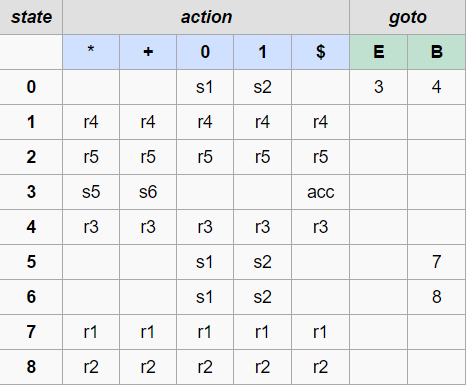
\includegraphics[width=0.5\textwidth]{LR-Table}
\caption{Example of LR grammar table. \cite{wikilr:online} }
\end{figure}
Generate this table, even if it can describe simply, was an important challenge and required a important effort. The current implementation works for simple case, but can produce wrong output for more complex grammar, even if it looks simple at first sight.

\subsection{Bottom-up parser : LR(0) Parser}
To implement my algorithm I had to implement a bottom-up parser. My choice was to implement a LR parser, principally because it's a key algorithm in most tools today, with a lot of variant as SLR, LR(1), LALR, GLR, ... \\
LR is the acronym for "Left input - Rightmost derivation" this kind of parser are really good to parser deterministic (at each state, we know which will be the next expected input) context free grammar and are mainly based on a grammar table as shown in the figure 1 and a stack\\
At each step, the stack will store the parse input and the state, so a stack in a LR parser can looks like :
\begin{lstlisting}[language=python, caption=example Lr parser stack]
stack = ['+', 1, '0', 0] # example of stack  
\end{lstlisting}
At each state, and in function of the parsed input the LR parser will know which action it have to do. Very few operation are done by a LR parser:
\begin{itemize}
\item Shift (ex: s1) : Shift (put the parse element in the stack) and push the state (here 1)
\item Reduce (ex: r1) : The reduce operation will remove element on the stack corresponding of the right-hand element of the rules indicate. (in the example the rule 1) and will look at the "goto" section on the table to know which state in the next
\item GoTo (ex: g3) : After a reduced operation, the next operation is a "go to" operation that will push the next state corresponding of the reduce rules. For example inside the figure 1, after a reduced operation that makes the parser go back to the state zero, the next state of the parser will be 3 if the reduce rules was E or 4 if it was B
\end{itemize}
This 3 operations are enough to parse any input, but the main work is done by the grammar table which know what to do next in function of the state and the next input.\\
This kind of parser is simple to implement IF the grammar table is provided, but the generation of the grammar table was a real challenge. Inside the implementation this algorithm work correctly for a correct grammar table.

\subsection{Top-down parser}
The top-down parser was easier to implement because I chose to implement a simpler parser than a LL one. I chose to implement the most basic top-down parser.\\
This implementation works pretty well, and can be used like this :
\begin{lstlisting}[language=java, caption=top-down parser example]
  var number = ((has('0') | has('1') | has('2'))["+"])..name = "num";
  var operator = (has('+') | has('-'))..name = "operator";
  var operation = (number & (((operator & number)..name="op")["*"]))..name = "operation";

  var expr = operation;
  var input = "12+2-1";
  var res = expr.check(input);
\end{lstlisting}

The current implementation rely on the grammar tree created. Each rule node have a 'check' method that allow to verify that the input match the rules, but if the node has a child, it will check its child first, and the child will check its own child, and so on... This will give the base of the top-down parsing algorithm. A better description of the algorithm used is :
\begin{lstlisting}[language=python, caption=top-down pseudo code algorithm]
 input = range of input between nb character match and the end of the input
 node = get next node
 nb_match = 0
 check match in child
 IF child match:
   check node match
   IF node match
      nb_match += 1
 IF nb_match is in node quantifier range:
   GO TO 4
 ELSE IF nb_match match node quantifier:
   RETURN number of character match
 ELSE:
   RETURN match_fail
\end{lstlisting}
 At each step, a MatchInfo is returned, storing all the information about the match as the number of character match, the rules who has been matched, the match input, ... This information are used to know the parser location inside the input, and to construct the syntax tree.\\
The main difference with a bottom-up algorithm is the starting point, in a bottom-up algorithm, the grammar is checked starting by the terminals rules, but in a top-down, the first rules checked is the root (or goal) rule.
 
\subsection{The combination algorithm}
The main idea was to combine this 2 algorithms depending of the context, sadly due to the complexity of implementing the LR algorithm and the time required in research to transform the grammar and generate the table was too much to allow me to correctly implement this algorithm.\\
All the pieces are here, the MatchInfo node allow me to know the location of each parsed information in the input, the size of the match, and so apply the potential correct algorithm. One of the challenge was to be able to generate the exact same tree, so it would have been possible to use one or the others in a seamless way.\\

\subsection{Missing \& Future functionality}
The actual implementation is not complete, due to some reason main features are not available :
\begin{itemize}
\item On-line edition
\item Research algorithm
\end{itemize}
This functionality has not been implemented due to the unexpected amount of time in research, test and comprehension some part of this project have required. The part on the grammar was a really hard part because grammar by itself is an entire field of research and the manipulation of the grammar to transform a syntax to an others is a complete field.\\
I have underestimate some part of the implementation too, as the time required to allow an "on-line" edition and so make the appropriate modifications to the syntax tree.